\documentclass[12pt]{article}
%\usepackage{alltt}
%\usepackage{helvet}
%\usepackage[sfdefault]{roboto}
\usepackage{amsmath}
\usepackage[utf8]{inputenc}
\usepackage[dvips]{graphicx}
%\usepackage{a4wide}
\usepackage{epsfig}
\usepackage{fancybox}
\usepackage{verbatim}
\usepackage{array}
\usepackage{latexsym}
\usepackage{alltt}
\usepackage{url}
\usepackage{color}   % added for colored text
%\usepackage{fullpage}
\usepackage{hyperref}
\usepackage{listings}
\usepackage{color}
\usepackage{calc}
\usepackage{enumitem}
\usepackage[hmargin=3cm,vmargin=5.0cm]{geometry}
%\topmargin=0cm
\topmargin=-1.8cm \addtolength{\textheight}{4.5cm}
\addtolength{\textwidth}{1.0cm}
%\setlength{\leftmargin}{-5cm}
\setlength{\oddsidemargin}{0.0cm}
\setlength{\evensidemargin}{0.0cm}

%\renewcommand{\familydefault}{\sfdefault}

\newcommand{\HRule}{\rule{\linewidth}{1mm}}
\newcommand{\kutu}[2]{\framebox[#1mm]{\rule[-2mm]{0mm}{#2mm}}}
\newcommand{\gap}{ \\[1mm] }

\newcommand{\Q}{\raisebox{1.7pt}{$\scriptstyle\bigcirc$}}

\definecolor{amaranth}{rgb}{0.9, 0.17, 0.31}
\definecolor{gray}{rgb}{0.4,0.4,0.4}
\definecolor{darkblue}{rgb}{0.0,0.0,0.6}
\definecolor{cyan}{rgb}{0.0,0.6,0.6}
\definecolor{red}{rgb}{0.6,0,0}
\definecolor{dkgreen}{rgb}{0,0.6,0}
\definecolor{mauve}{rgb}{0.58,0,0.82}
\definecolor{lightblue}{rgb}{0.0,0.0,0.9}
\definecolor{darkred}{rgb}{0.6,0.0,0.0}

\lstset{
    %backgroundcolor=\color{lbcolor},
    tabsize=4,
    basicstyle=\fontsize{10}{10.3}\selectfont\sffamily,
    numberstyle=\footnotesize,
    aboveskip={0.0\baselineskip},
    belowskip={0.0\baselineskip},
    columns=fullflexible,
    breaklines=true,
    prebreak=\raisebox{0ex}[0ex][0ex]{\ensuremath{\hookleftarrow}},
    frame=single,
    showtabs=false,
    showspaces=false,
    showstringspaces=false,
    identifierstyle=\color{amaranth},
    keywordstyle=\color{rgb}{0,0,1},
    commentstyle=\color[rgb]{0.133,0.545,0.133},
    stringstyle=\color{amaranth},
}

\lstdefinelanguage{XML}
{
  morestring=[s][\color{red}]{"}{"},
  morestring=[s][\color{black}]{>}{<},
  morecomment=[s]{<?}{?>},
  morecomment=[s][\color{dkgreen}]{<!--}{-->},
  %stringstyle=\color{black},
  identifierstyle=\color{black},
  keywordstyle=\color{darkblue},
  commentstyle=\color[rgb]{0.133,0.545,0.133},
  stringstyle=\color{black},
  morekeywords={Scene,BackgroundColor,ShadowRayEpsilon,
  MaxRecursionDepth,Cameras,Camera,Position,Gaze,Up,
  NearPlane,NearDistance,ImageResolution,ImageName,
  Material,Materials,VertexData,Mesh,Triangle,Sphere,
  Faces,Lights,AmbientLight,PointLight,Objects,Indices,
  AmbientReflectance,DiffuseReflectance,SpecularReflectance,PhongExponent,MirrorReflectance,Intensity,Center,Radius,xmlns,version}% list your attributes here
}

\begin{document}

\noindent \HRule \\[3mm]
\small
\begin{tabular}[b]{lp{1.2cm}r}
\href{https://www.metu.edu.tr/}{
\epsfig{file=metulogo.eps,width=5mm}} Middle East Technical
University &  &
\href{https://ceng.metu.edu.tr/information}{
\epsfig{file=bmblogo.eps,width=5mm}} Department of Computer Engineering \\
\end{tabular} \\
\begin{center}

                 \LARGE \textbf{CENG 795} \\[4mm]
                 \Large Advanced Ray Tracing \\[4mm]
                \normalsize Fall '2022-2023 \\
                    \normalsize Assignment 6 - Putting it All Together:
                    BRDFs and Path Tracing\\
                    \normalsize (v.1.0)
\end{center}
\HRule

\begin{center}
Due date: January 22, 2022, Sunday, 23:59
\end{center}

\centerline{
    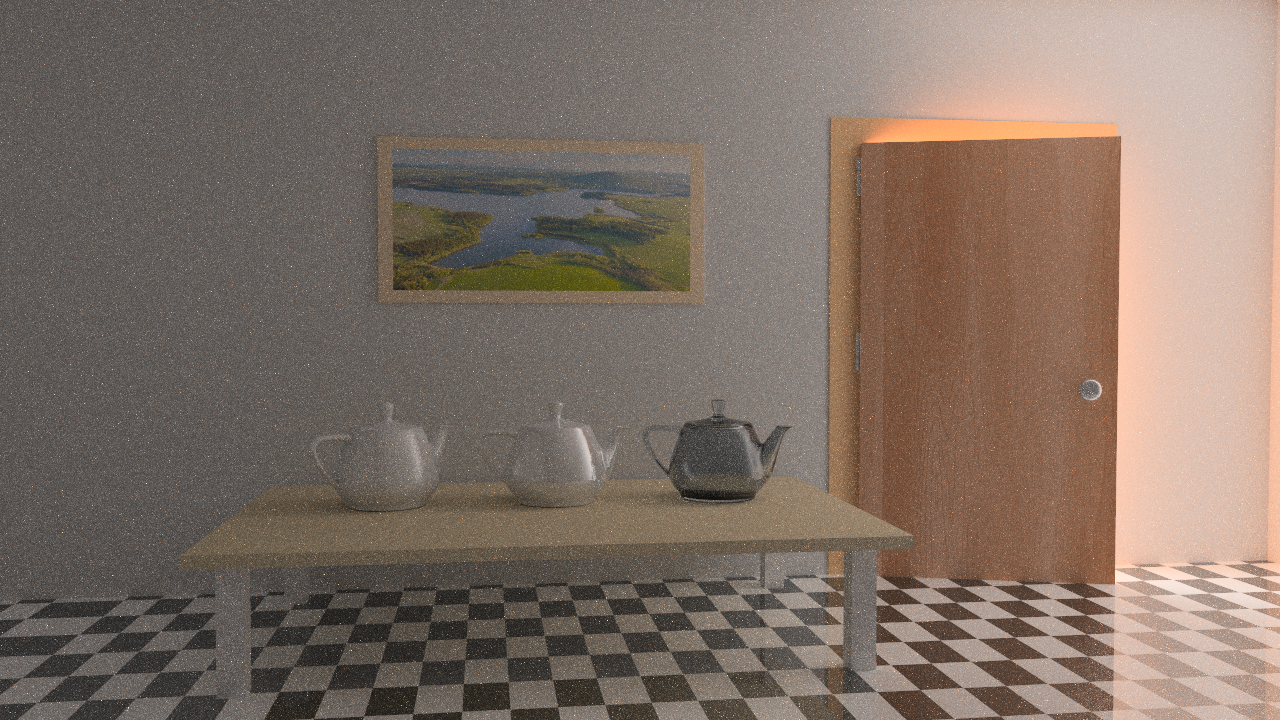
\includegraphics[width=5in]{../veach-ajar/outputs/VeachAjar_path.png}
}

\section{Objectives}

In this homework we are going to bring together all the things that we
learned so far to implement a fully functional path tracer. In
particular the features that you will implement are:

\begin{itemize}
    \item BRDF models
    \item Object lights
    \item Path tracing with uniform and important sampling
\end{itemize}

\vspace{0.5cm} \noindent \textbf{Keywords:} \emph{path tracing, BRDF,
    importance sampling}

\section{Specifications}

The specifications are the same as for the previous homeworks so are not
repeated here. Make sure you check out the supporting PDF files that are
separately uploaded in case you need extra clarifications.

\section{Scene File}
\label{sec:sceneFile}

\subsection{BRDF}

A BRDF will be defined in the scene file as follows:

\begin{verbatim}
<BRDFs>
    <ModifiedBlinnPhong id="1" normalized="true">
        <Exponent>50</Exponent>
    </ModifiedBlinnPhong>
</BRDFs>
\end{verbatim}

Possible BRDF types are:
%
\begin{itemize}
\item OriginalBlinnPhong (this is the BRDF of the default shading model we have been using so far)
\item OriginalPhong
\item ModifiedBlinnPhong (can be normalized as shown above)
\item ModifiedPhong (can be normalized)
\item TorranceSparrow (normalized by definition)
\end{itemize}
%
For the Torrance-Sparrow BRDF the exponent is the $p$ term used in the
distribution function. For that BRDF, there is an attribute called
\emph{kdfresnel}. If this is true, it means that you should use
$\frac{(1 - F)k_d}{\pi}$ instead of $\frac{k_d}{\pi}$ when computing the
diffusely reflected radiance.  Please refer to the BRDF document for specific
details.

\subsection{Object Lights}

Any regular object can now be a light source. For example, we can make a
sphere light source by defining it as \texttt{LightSphere}:
%
\begin{verbatim}
<LightSphere id="1">
    <Material>1</Material>
    <Center>11</Center>
    <Radius>0.2</Radius>
    <Radiance>31.831 31.831 31.831</Radiance>
</LightSphere>
\end{verbatim}
%
This is the same definition as a regular sphere except that it also has
a radiance element. A mesh light is similar:
%
\begin{verbatim}
<LightMesh id="1">
    <Faces> 2 6 7 7 3 2 </Faces>
    <Material>1</Material>
    <Radiance>1.21 1.21 1.21</Radiance>
</LightMesh>
\end{verbatim}
%
Note that in case of pure path tracing, you do not have to do anything
special to sample an object light. Some rays will simply hit them and
get the corresponding radiance value (still divided by the probability
of uniform or importance sampling). But if you are doing explicit
light sampling (also known as \emph{next event estimation}), you must
sample a point on the light source and divide the returned radiance
value by the probability of sampling the corresponding direction. 

\subsection{Path Tracing}

Until now, we sent a recursive ray only when an object was a mirror,
conductor, or dielectric. With path tracing, we send recursive
rays for all types of objects. This is because in reality all
objects exchange light with each other. We may call these
recursively sent rays as global or indirect illumination rays.
This way if only a part of the scene receives direct illumination,
the scene will still be illuminated because that part will reflect
light to other parts. 

With path tracing, we typically disable the
crude ambient term we used so far. Instead, each scene point
receives some ambient light depending on its geometric
relationship to other objects in the scene. In the teaser figure
shown at the top, almost everywhere would be black without path
tracing because there is almost no direct illumination: all the
light comes from a small opening behind the door (hence the name
\emph{ajar}).

Path tracing mode is enabled through the addition of the following XML
elements to the \texttt{Camera} element:
%
\begin{verbatim}
<Renderer>PathTracing</Renderer>
<RendererParams>NextEventEstimation ImportanceSampling RussianRoulette</RendererParams>
\end{verbatim}
%
So we can define multiple cameras, each camera with a different renderer
setting. The \texttt{RendererParams} element is optional. If it is
missing or empty, it means path tracing with uniform sampling. Otherwise
it may contain the following options:
%
\begin{itemize}
\item Importance Sampling: you must use cosine based
sampling of the upper hemisphere instead of uniform sampling.
\item Next Event Estimation: you must directly sample light sources in
addition to random sampling (see below)
\item Russian Roulette: you must terminate ray paths probabilistically
rather than using a fixed recursion depth (see below)
\end{itemize}
%
In next event estimation, for each primary ray we perform two operations:
(1) Sample a direction that will hit a light source (in case of an
occluder the hit may not happen, but this is not relevant) and (2)
sample a random global illumination ray. If the global illumination ray
happens to hit the same light source that you explicitly sampled in (1),
you must discard its contribution. Otherwise, you count a light twice
and introduce bias in your result.

Russian roulette is a dangerous game for humans and rays alike. The idea
is to probabilistically terminate a ray path if it is likely to make a
low contribution.  For example, after many bounces the impact of the ray
will significantly diminish because each bounce will absorb the energy
of the ray. Assume that initially the ray has a \emph{throughput} of
$1$. If a ray bounces from a surface along a direction whose BRDF is
$0.2$, its throughput will be $0.2$. Now if the ray bounces again from
another surface with a BRDF of $0.1$, the new throughput will be $0.02$.
This means, whatever radiance that may come from the direction of the
ray from this point on, it will get scaled by a factor of $0.02$. So we
can use this throughput factor to probabilistically terminate the ray. 
The steps to implement Russian roulette are as follows:
%
\begin{enumerate}
\item Draw a normalized uniform number, $\xi$
\item If $\xi > q$ where $1 - q$ is the termination probability, kill the
rest of this path (e.g., if $q = 0.9$, the ray will be terminated with
$0.1$ probability). You can use any $q$ you want but using throughput is
a sensible choice: low throughput paths are more likely to be killed than
high throughput paths.
\item Add a constant term $C$ to model the radiance that we may have
lost due to terminating the path. $C = 0$ is a common choice.
\item Compute the final estimate as a weighted average of the computed
estimate and the ignored estimate:
%
\begin{align}
F' =
\begin{cases}
\frac{F - (1 - q)C}{q}, & \xi \le q \\
C, & \xi > q
\end{cases}
\end{align}
%
Note that the expected value of $F'$ is the same as the expected value
of $F$.
\end{enumerate}
%
Note that variance will generally increase with Russian roulette - so it
is not a variance reduction technique. But it gives us a statistically
sound way to terminate rays instead of cutting them after a fixed number
of bounces.  In general, it is best to combine it with the maximum
recursion depth parameter: kill the ray if it fails the throughput test
\emph{and} it exceeds the maximum recursion depth. However, the scene
results shared with you do not implement this technique -- only the
direct application of Russian roulette is shown, therefore results are
generally noisier.

\section{Hints \& Tips}
In addition to those for the previous homeworks, the following tips may
be useful for this homework.

\begin{enumerate}

\item There are a few scenes among the input files that
will make you grateful for having implemented an acceleration
structure, but regretful that you haven't optimized it further.

\item You can stratify your global illumination ray samples for reducing
variance.

\item If you want, you can send multiple global illumination ray samples
for each primary ray sample. But the shared results are created by sending one
illumination sample per primary ray sample.

\item The sponza scene contains vertex and texture data in binary files.
For vertex data it is just $x, y, z$ values of each vertex packed
together. You must open these files in binary more to read them
correctly. For texture data, it is the $u, v$ values packed in the same
manner. For index data, it is the integer index values. Each binary data
starts with a single integer value that represents the number of
elements to read. For vertex data, it is the number of vertices. For
texture data, it is the number of texture coordinates. For index data,
it is the number of faces (in this case you must read three times of
this value as each face is represented using $3$ indices).

\item If you come across
\texttt{<ZeroBasedIndexing>true</ZeroBasedIndexing>} element in the XML
file, you must assume that indices are zero-based as opposed to the
one-based convention that we have been using.

\item Similarly, if you come across \texttt{vertexOffset} or
\texttt{textureOffset} attributes in face definitions, it means you
must add these amounts to the indices before accessing the vertex and
texture data. Note that these numbers can be negative!

\end{enumerate}

\section{Bonus}

I will give a significant bonus to students who convert some complex
PBRT (\url{https://github.com/mmp/pbrt-v4-scenes}) or Tungsten
(\url{https://benedikt-bitterli.me/tungsten.html}) scenes to our format
and render them correctly.

\section{Regulations}

\begin{enumerate}

\item \textbf{Programming Language:} C/C++ is the recommended language.
However, other languages can be used if so desired. In the past, some
some students used Rust or even Haskell for implementing their ray
tracers.

\item \textbf{Changing the Sample Codes:} You are free to modify any
sample code provided with this homework.

\item \textbf{Additional Libraries:} If you are planning to use any
library other than \textit{(i)} the standard library of the language,
\textit{(ii)} pthread, \textit{(iii)} the XML parser, and the PNG
libraries please first ask about
it on ODTUClass and get a confirmation. Common sense rules apply: if a
library implements a ray tracing concept that you should be
implementing yourself, do not use it!

\item \textbf{Submission:} Submission will be done via ODTUClass. 
To submit, Create a
``\textbf{tar.gz}''  file  named  ``raytracer.tar.gz'' that
contains all your source code files and a Makefile. The
executable should  be  named as  ``raytracer'' and  should  be
able  to  be  run  using  the following commands (scene.xml
        will be provided by us during grading):\\

\indent \textbf{tar -xf raytracer.tar.gz}\\
\indent \textbf{make}\\
\indent \textbf{./raytracer scene.xml}\\

\noindent Any error in these steps will cause point penalty during
grading.

\item \textbf{Late Submission:} You can submit your codes up to 3 days
late. Each late day will cause a 10 point penalty.

\item \textbf{Cheating:} \textbf{We have zero tolerance policy
for cheating}.  People involved in cheating will be
punished according to the university regulations and will
get 0 from the homework. You can discuss algorithmic choices,
but sharing code between groups or using third party code
is strictly forbidden. By the nature of this class, many past students
make their ray tracers publicly available. You must refrain from using
them at all costs.

\item \textbf{Forum:} Check the ODTUClass forum regularly for
updates/discussions.

\item \textbf{Evaluation:} The basis of evaluation is your blog posts.
Please try to create interesting and informative blog posts about your
ray tracing adventures. You can check out various past blogs for
inspiration. However, also expect your codes to be compiled and tested
on some examples for verification purposes. So the images that you share
in your blog post must directly correspond to your ray tracer outputs.

\end{enumerate}

\end{document}
